\documentclass[tikz]{standalone}
\usepackage{pgfplots}
\pgfplotsset{compat=1.18}

\begin{document}
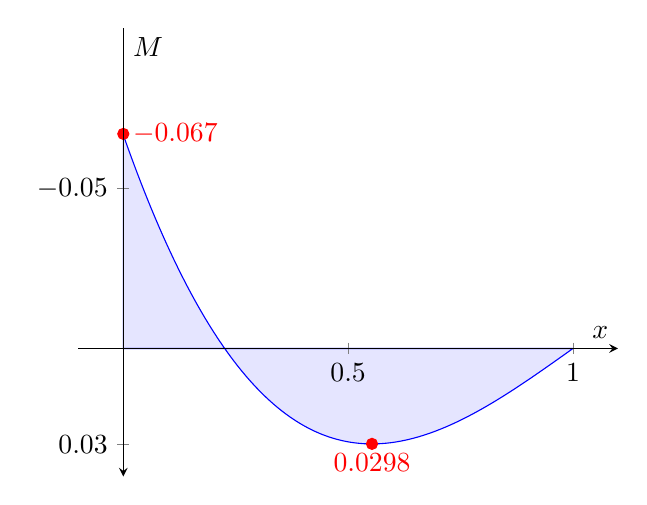
\begin{tikzpicture}
	\begin{axis}[
		axis lines = middle,
		xlabel = $x$,
		ylabel = {$M$},
		y dir = reverse,
		xmin=-.1, xmax=1.1,
		ymin=-.1, ymax=0.04,
		xtick= {0.5, 1},
		ytick= {-0.05, 0, 0.03},  %  Añade algunos valores para el eje y
		yticklabel style={/pgf/number format/fixed}, % Formato numérico fijo
		set layers, % Activa las capas
		axis on top
		]
		\addplot [
		domain=0:1, 
		samples=100, 
		color=blue,
		fill=blue!10,
		]
		{-1/15 + 2/5*x - x^2/2 + x^3/6} \closedcycle;
		
		% Punto máximo
		\addplot[mark=*, color=red] coordinates {(0.553,0.0298)} node[below] {$0.0298$};
		
		% Punto mínimo
		\addplot[mark=*, color=red] coordinates {(0,-0.067)} node[right] {$-0.067$}; 
	\end{axis}
\end{tikzpicture}
\end{document}